\subsection{Support Vector Machines}
Support vector machines try to separate data in a multidimensional space into a subset of classes using a hyperplane.
Here the most common three kernels for SVMs will be considered.
These are, the Gaussian Radial Basis, the Polynomial and Linear kernel.

Below the optimum parameters for the Gaussian Radial Basis and the Polynomial kernel will be found.
As the Linear kernel does not have any parameters to change, it will be used directly in the test.

\subsubsection{Gaussian Radial Basis Kernel}
The Gaussian Radial Basis Kernel (RBF) function is given in equation \ref{eq:rbf}.

\begin{equation}
k(x,x') = \exp(-\sigma \|x - x'\|^2)
\label{eq:rbf}
\end{equation}

In figure \ref{fig:rbf} the result for the person independent test of G3M2 is shown when sigma goes from 0 to 6.
Only one person is used to decide the parameter in order to reduce processing time.

\begin{figure}[H]
\centering
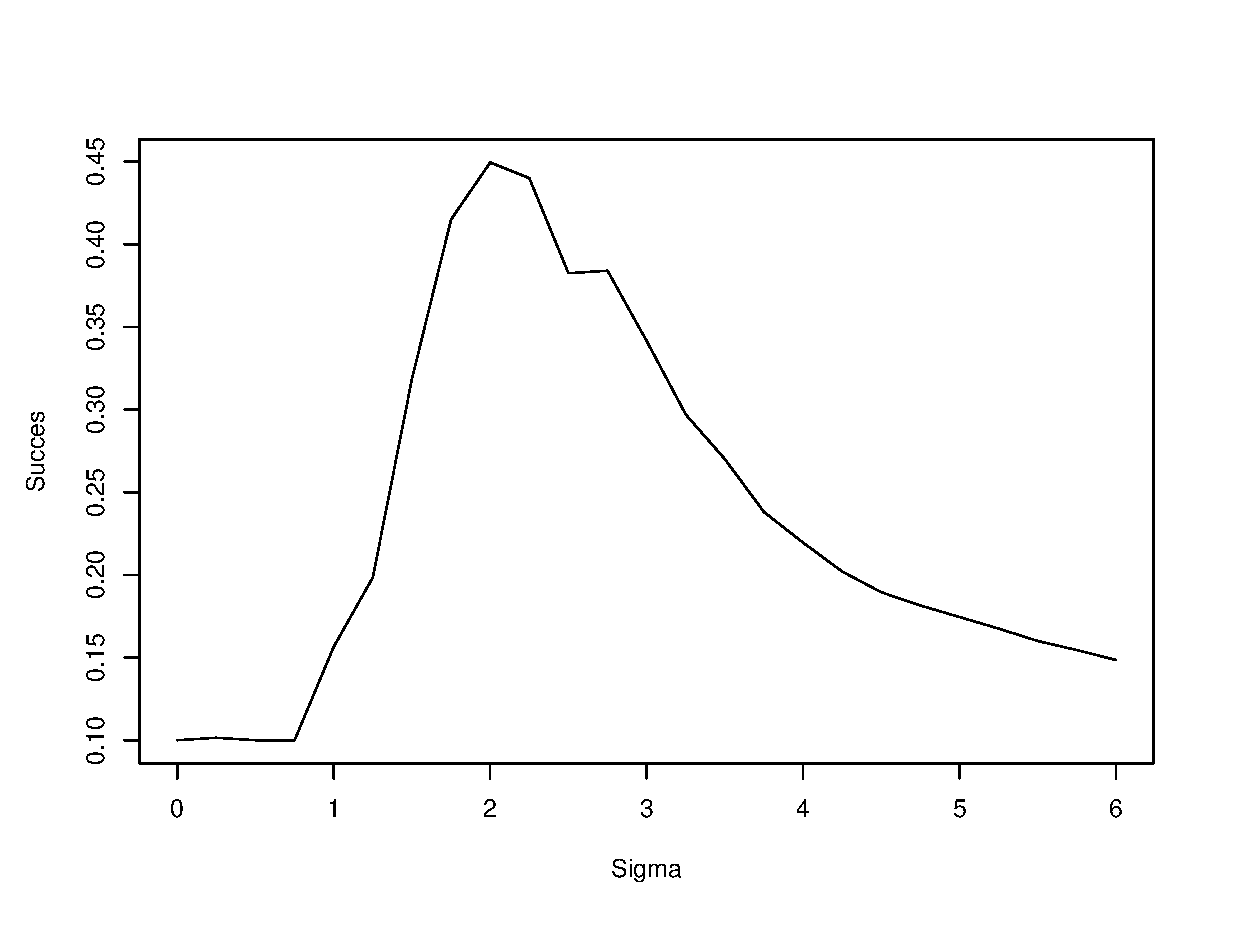
\includegraphics[width = 0.9 \textwidth]{graphics/lineplot_svm_rbf}
\caption{Kernel success rate for different sigma values when using the Gaussian Radial Basis kernel.}
\label{fig:rbf}
\end{figure}

From figure \ref{fig:rbf} the optimum point can be found to be $\sigma = 2$.

\subsubsection{Polynomial Kernel}
The equation for the polynomial kernel is given in equation \ref{eq:poly}.

\begin{equation}
k(x,x') = (scale <x, x'> +\ offset)^{degree}
\label{eq:poly}
\end{equation}

As seen in equation \ref{eq:poly}, then the polynomial function has 3 parameters to adjust.
These are the scale, offset and degree.
To simplify the selection of the optimum parameters, it was decided only to consider the scale and degree and use the default value for offset.
In figure \ref{fig:poly} the success for the person independent test of G3M2 is shown when the degree and scale goes from 1 to 4 and 0 to 0.08 respectively.

\begin{figure}[H]
\centering
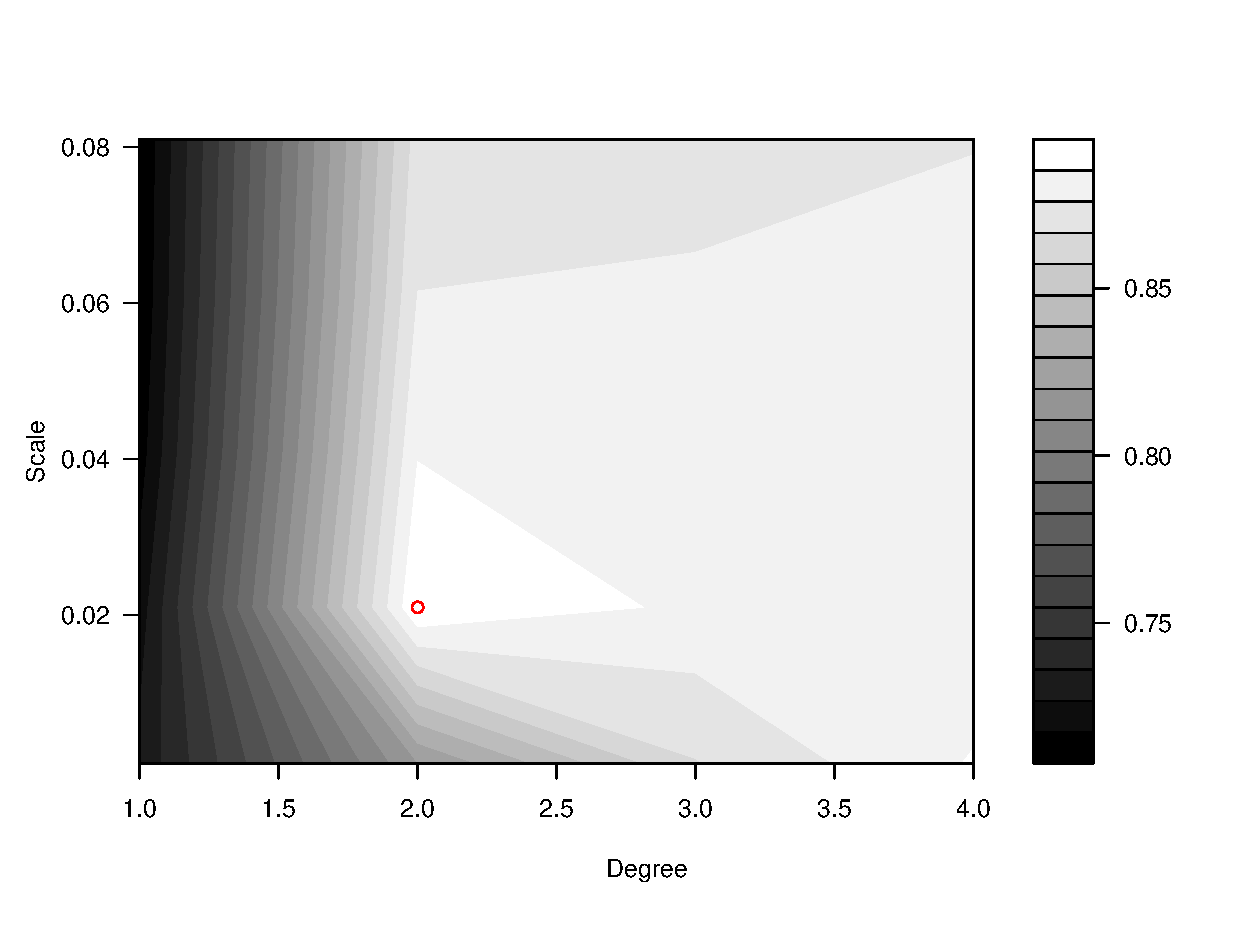
\includegraphics[width = 0.9 \textwidth]{graphics/contour_svm_poly}
\caption{Kernel success rate for different orders and scale values when using the poly kernel.
The red circle marks the point of which the success was found to be the maximum.}
\label{fig:poly}
\end{figure}

It was from figure \ref{fig:poly} found that the optimum scale and degree is 0.02 and 2 respectively when the default offset is used.


\subsubsection{Kernel Comparison}
The comparison of the three kernels can be seen in figure \ref{fig:comp_kernel}.
The Gaussian RBF was run with a sigma of 2 and the polynomial function a degree and scale of 2 and 0.02 respectively.


\begin{figure}[H]
\centering
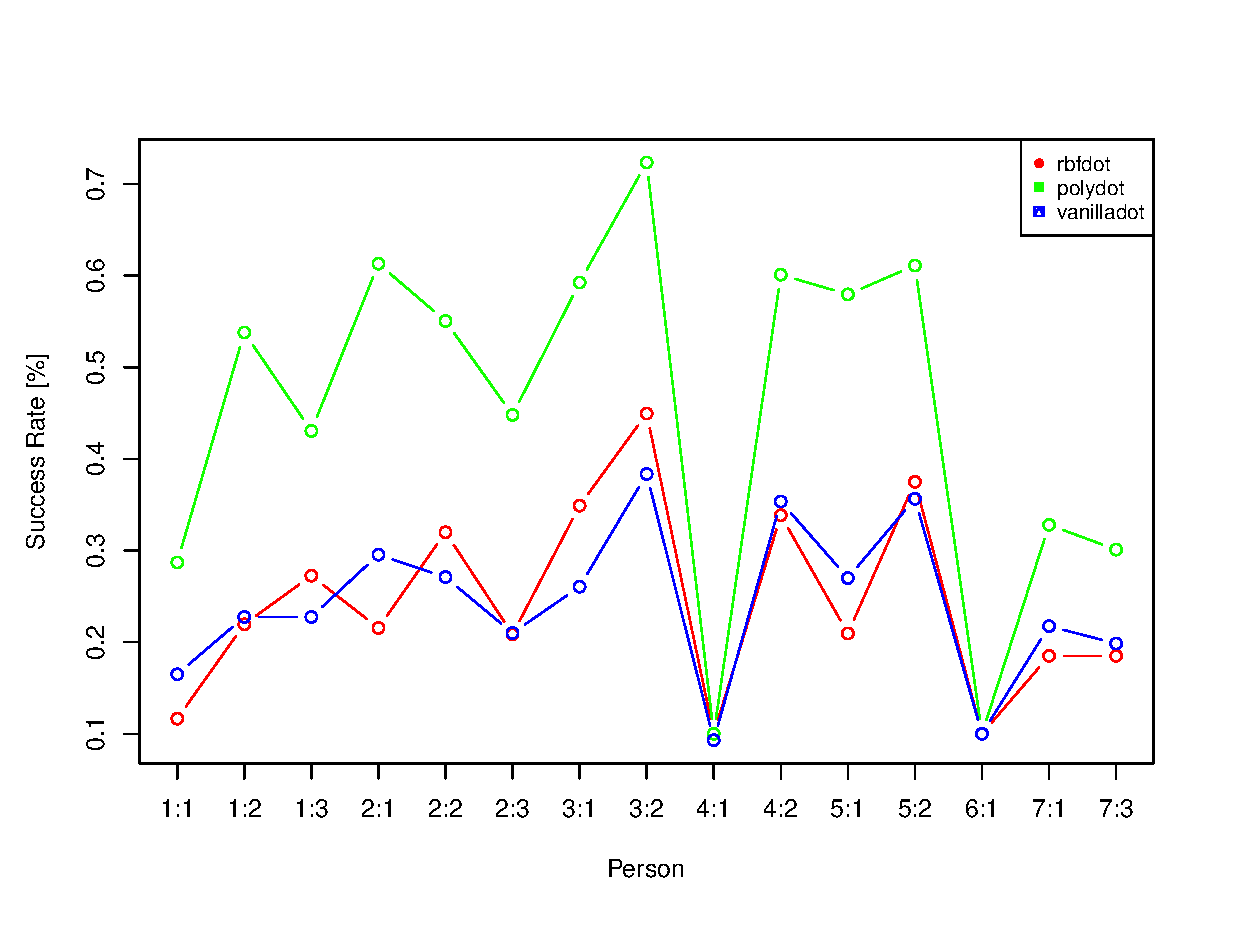
\includegraphics[width = \textwidth]{graphics/svm_kernel_comp}
\caption{Comparison of 15 independent datasets and the SVM kernel used. The mean success rate of the datasets are shown in table \ref{tab:mean_succes_kernel}.}
\label{fig:comp_kernel}
\end{figure}

%"mean rbf: 0.242933333333333
%"mean poly: "       "0.453566666666667"
%"mean vanilla: "    "0.241966666666667"

\begin{table}[H]
\centering
\begin{tabular}{|l|c|}
\hline
Kernel & Mean Success\\ \hline
RBF & 24.29 \% \\ \hline
Polynomial & 45.36 \% \\ \hline
Vanilla & 24.20 \% \\ \hline
\end{tabular}
\caption{Mean success rate of figure \ref{fig:comp_kernel}.}
\label{tab:mean_succes_kernel}
\end{table}


As seen on figure \ref{fig:comp_kernel} and in table \ref{tab:mean_succes_kernel}, then the polynomial kernel is performing almost twice as good as the two other kernels for this classification problem.
%The two sudden drops in success in figure \ref{fig:comp_kernel} at 4:1 and 6:1 are surprising because of their success of all three kernels being approximately equal, but it is not possible for us to explain why this is the case.

